\documentclass[11pt,compress,t,notes=noshow]{beamer}
\usepackage[]{graphicx}\usepackage[]{color}
% maxwidth is the original width if it is less than linewidth
% otherwise use linewidth (to make sure the graphics do not exceed the margin)
\makeatletter
\def\maxwidth{ %
  \ifdim\Gin@nat@width>\linewidth
    \linewidth
  \else
    \Gin@nat@width
  \fi
}
\makeatother

\definecolor{fgcolor}{rgb}{0.345, 0.345, 0.345}
\newcommand{\hlnum}[1]{\textcolor[rgb]{0.686,0.059,0.569}{#1}}%
\newcommand{\hlstr}[1]{\textcolor[rgb]{0.192,0.494,0.8}{#1}}%
\newcommand{\hlcom}[1]{\textcolor[rgb]{0.678,0.584,0.686}{\textit{#1}}}%
\newcommand{\hlopt}[1]{\textcolor[rgb]{0,0,0}{#1}}%
\newcommand{\hlstd}[1]{\textcolor[rgb]{0.345,0.345,0.345}{#1}}%
\newcommand{\hlkwa}[1]{\textcolor[rgb]{0.161,0.373,0.58}{\textbf{#1}}}%
\newcommand{\hlkwb}[1]{\textcolor[rgb]{0.69,0.353,0.396}{#1}}%
\newcommand{\hlkwc}[1]{\textcolor[rgb]{0.333,0.667,0.333}{#1}}%
\newcommand{\hlkwd}[1]{\textcolor[rgb]{0.737,0.353,0.396}{\textbf{#1}}}%
\let\hlipl\hlkwb

\usepackage{framed}
\makeatletter
\newenvironment{kframe}{%
 \def\at@end@of@kframe{}%
 \ifinner\ifhmode%
  \def\at@end@of@kframe{\end{minipage}}%
  \begin{minipage}{\columnwidth}%
 \fi\fi%
 \def\FrameCommand##1{\hskip\@totalleftmargin \hskip-\fboxsep
 \colorbox{shadecolor}{##1}\hskip-\fboxsep
     % There is no \\@totalrightmargin, so:
     \hskip-\linewidth \hskip-\@totalleftmargin \hskip\columnwidth}%
 \MakeFramed {\advance\hsize-\width
   \@totalleftmargin\z@ \linewidth\hsize
   \@setminipage}}%
 {\par\unskip\endMakeFramed%
 \at@end@of@kframe}
\makeatother

\definecolor{shadecolor}{rgb}{.97, .97, .97}
\definecolor{messagecolor}{rgb}{0, 0, 0}
\definecolor{warningcolor}{rgb}{1, 0, 1}
\definecolor{errorcolor}{rgb}{1, 0, 0}
\newenvironment{knitrout}{}{} % an empty environment to be redefined in TeX

\usepackage{alltt}
\newcommand{\SweaveOpts}[1]{}  % do not interfere with LaTeX
\newcommand{\SweaveInput}[1]{} % because they are not real TeX commands
\newcommand{\Sexpr}[1]{}       % will only be parsed by R



\usepackage[english]{babel}
\usepackage{dsfont}
\newcommand\bmmax{2}
\usepackage{bm}
\usepackage{bbm}
\usepackage{verbatim}
\usepackage{amsmath}
\usepackage{amsfonts}
\usepackage{csquotes}
\usepackage{multirow}
\usepackage{longtable}
\usepackage{enumerate}
\usepackage[absolute,overlay]{textpos}
\usepackage{psfrag}
\usepackage{algorithm}
\usepackage{algorithmicx}
\usepackage{algpseudocode}
\usepackage{eqnarray}
\usepackage{multimedia}
\usepackage{media9}
\usepackage{arydshln}
\usepackage{tabularx}
\usepackage{placeins}
\usepackage{tikz}
\usepackage{setspace}
\usepackage{wrapfig}
\usepackage{tcolorbox}
\usepackage[export]{adjustbox}
\usepackage{siunitx}
\usetikzlibrary{shapes,arrows,automata,positioning,calc}
\tikzset{
  %Define standard arrow tip
  >=stealth',
  %Define style for boxes
  punkt/.style={
    rectangle,
    rounded corners,
    draw=black, very thick,
    text width=6.5em,
    minimum height=2em,
    text centered},
  % Define arrow style
  pil/.style={
    ->,
    thick,
    shorten <=2pt,
    shorten >=2pt,}
}
\usepackage{subfig}

%new environments

\newenvironment{vbframe}  %frame with breaks and verbatim
{
 \begin{frame}[containsverbatim,allowframebreaks]
}
{
\end{frame}
}

\newenvironment{vframe}  %frame with verbatim without breaks (to avoid numbering one slided frames)
{
 \begin{frame}[containsverbatim]
}
{
\end{frame}
}

\newenvironment{blocki}[1]   % itemize block
{
 \begin{block}{#1}\begin{itemize}
}
{
\end{itemize}\end{block}
}

\newenvironment{fragileframe}[2]{  %fragile frame with framebreaks
\begin{frame}[allowframebreaks, fragile, environment = fragileframe]
\frametitle{#1}
#2}
{\end{frame}}


\newcommand{\myframe}[2]{  %short for frame with framebreaks
\begin{frame}[allowframebreaks]
\frametitle{#1}
#2
\end{frame}}

\newcommand{\remark}[1]{
  \textbf{Remark:} #1
}

%%%%%%%%%%%%%%%%%%%%%%%%%%%%%%%%%%%%%%%%%%%%%%%%%%%%%%%%%%%%%%%%%%%%%%%%%%%%%%%

% basic latex stuff
\newcommand{\pkg}[1]{{\fontseries{b}\selectfont #1}} %fontstyle for R packages
\newcommand{\lz}{\vspace{0.5cm}} %vertical space
\newcommand{\dlz}{\vspace{1cm}} %double vertical space
\newcommand{\oneliner}[1] % Oneliner for important statements
{\begin{block}{}\begin{center}\begin{Large}#1\end{Large}\end{center}\end{block}}


%\usetheme{lmu-lecture}
\usepackage{../style/lmu-lecture}

\let\code=\texttt
\let\proglang=\textsf

\setkeys{Gin}{width=0.9\textwidth}



\title{Deep Learning}
\author{Mina Rezaei}
\institute{Department of Statistics -- LMU Munich}
\date{Winter Semester 2020}

\setbeamertemplate{frametitle}{\expandafter\uppercase\expandafter\insertframetitle}



\begin{document}

    
    \input{../../latex-math/basic-math}
\input{../../latex-math/basic-ml}
\input{../../latex-math/ml-nn}

\lecturechapter{5}{Application of CNNs}
\lecture{Deeplearning}

%%%%%%%%%%%%%%%%%%%%%%%%%%%%%%%%%%%%%%%%%%%%%%%%%%%%%%%%%%%%%%%%%%

\begin{frame}
\frametitle{Lecture outline}
\tableofcontents
\end{frame}
%%%%%%%%%%%%%%%%%%%%%%%%%%%%%%%%%%%%%%%%%%%%%%%%%%%%%%%%%%%%%%%%%%
    \section{Different Perspectives of CNNs}
%%%%%%%%%%%%%%%%%%%%%%%%%%%%%%%%%%%%%%%%%%%%%%%%%%%%%%%%%%%%%%%%%%
    \begin{vbframe}{CNNs - Perspective I}
\center
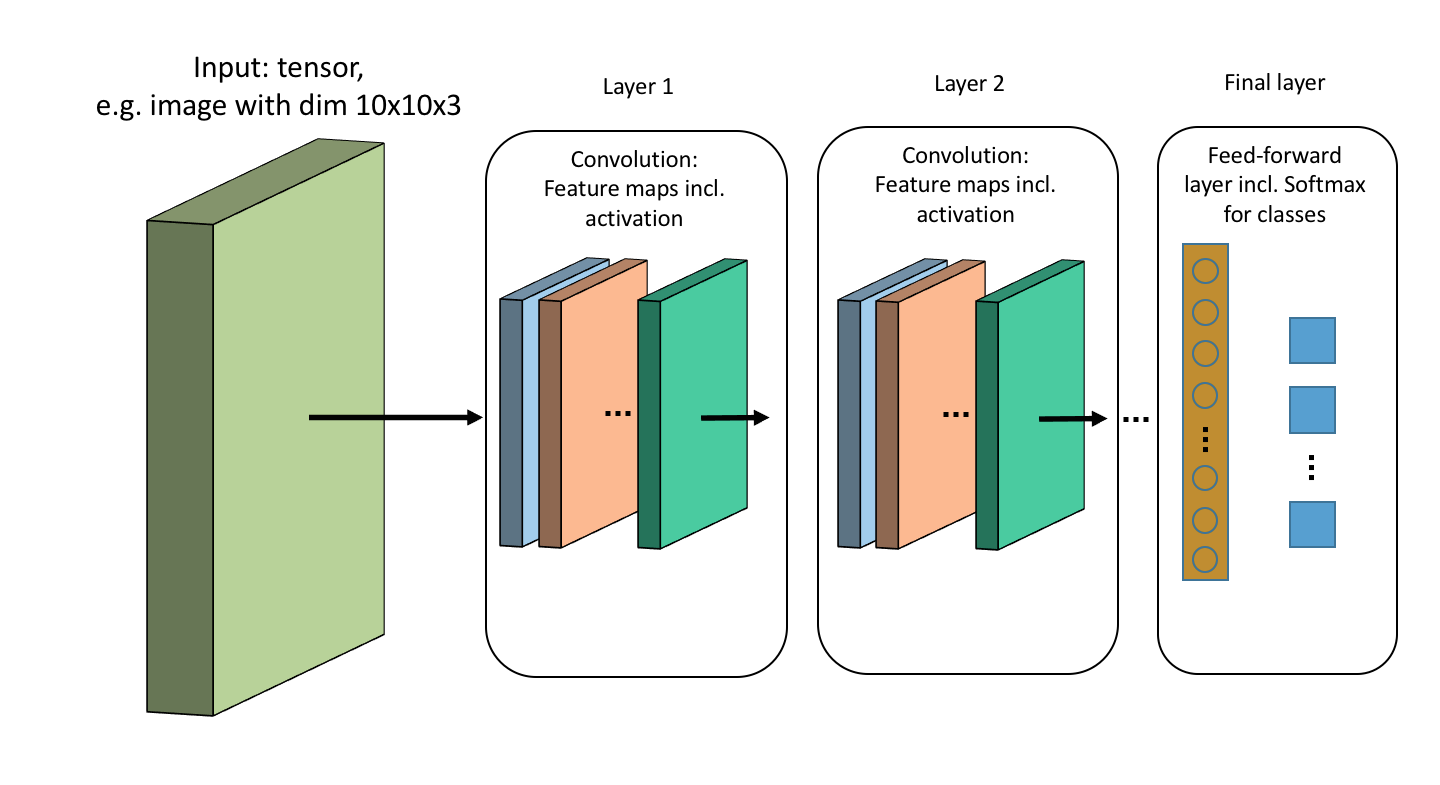
\includegraphics[width=9cm]{plots/03_first_glimpse/cnn_scheme.png}
\begin{itemize}
\item Schematic architecture of a CNN.
\item The input tensor is convolved by different filters yielding different feature maps (coloured) in subsequent layers.
\item A dense layer connects the final feature maps with the softmax-activated output neurons.
\end{itemize}
\end{vbframe}

\begin{vbframe}{CNNs - Perspective II}
\center
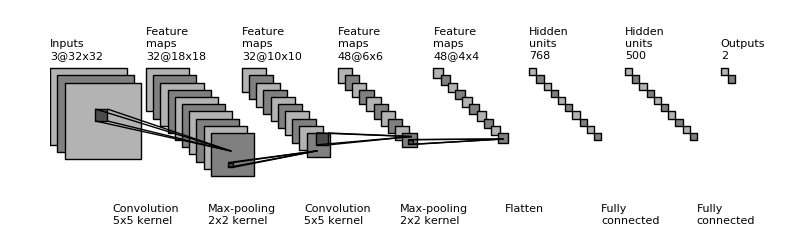
\includegraphics[width=11cm]{plots/03_first_glimpse/cnn_flat.png}
\begin{itemize}
\item Flat view of a CNN architecture for a classification problem.
\item Consists of 2 CNN layers that are each followed by max-pooling, then flattened and connected with the final output neurons via a dense layer.
\end{itemize}
\end{vbframe}

\begin{vbframe}{CNNs - Perspective III}
\center
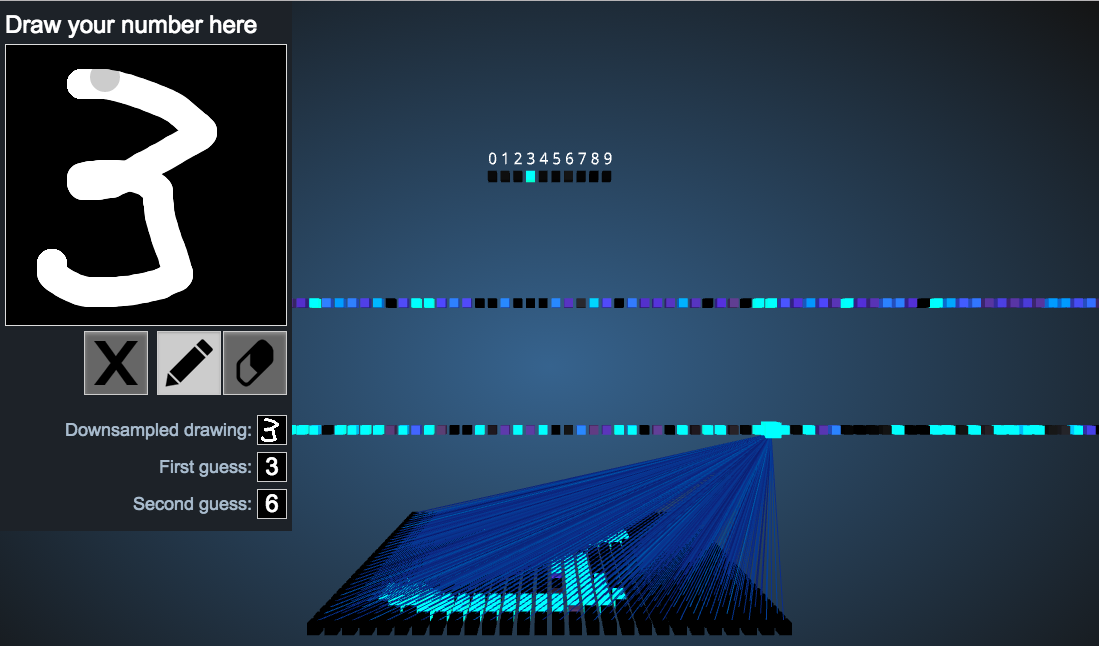
\includegraphics[width=8cm]{plots/03_first_glimpse/3dviz_fcn.png}
\begin{itemize}
% \item Awesome interactive visualization by \cite{29} (\href{http://scs.ryerson.ca/~aharley/vis/}{click here})
\item Awesome interactive visualization (by Adam Harley)  \href{http://scs.ryerson.ca/~aharley/vis/}{\beamergotobutton{Click here}}.
\item Vanilla 2-layer densely-connected net on MNIST data for input digit $3$.
\item Each neuron in layer 1 is connected to each of the input neurons.
\end{itemize}
\framebreak
\center
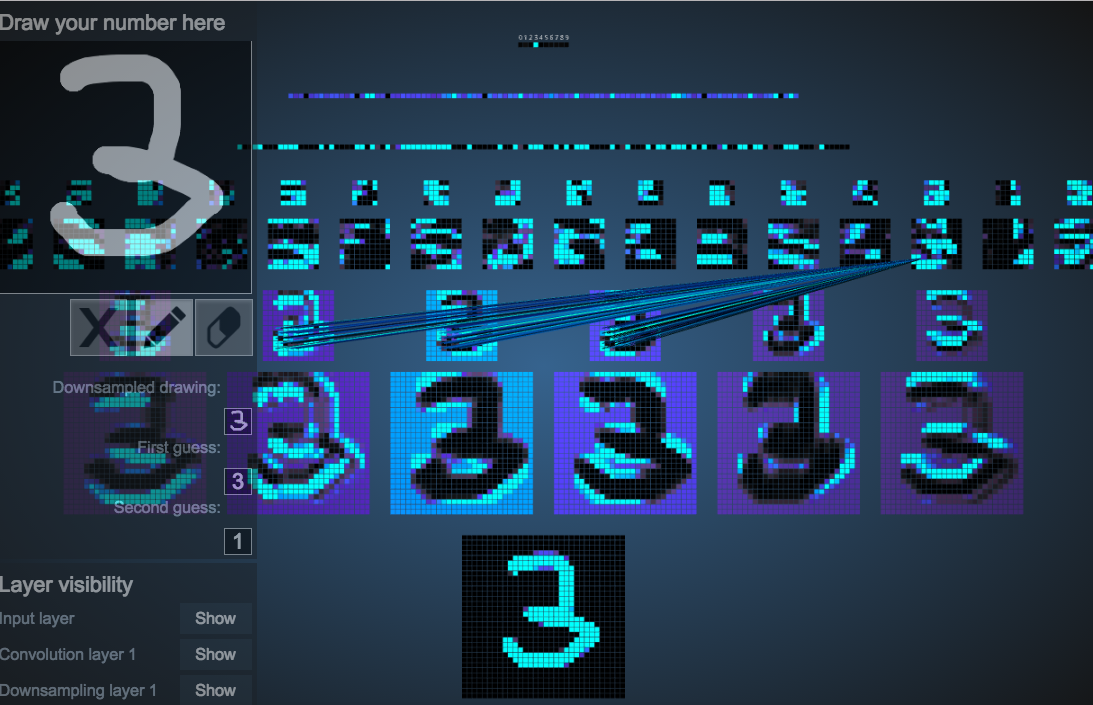
\includegraphics[width=8cm]{plots/03_first_glimpse/3dviz_cnn_front.png}
\begin{itemize}
\item Front view on 2-layer CNN with Pooling and final dense layer on MNIST data for input digit $3$.
\item Each neuron in the second CNN layer is connected to a patch of neurons from each of the previous feature maps via the convolutional kernel.
\end{itemize}
\framebreak
\center
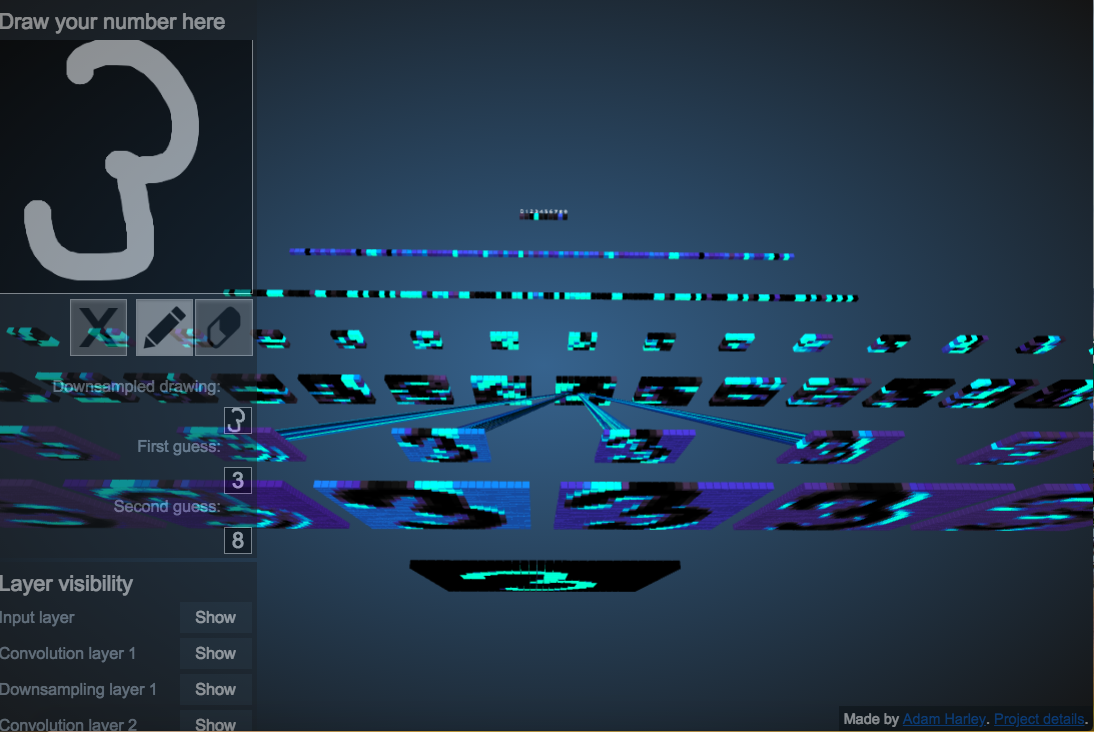
\includegraphics[width=7.5cm]{plots/03_first_glimpse/3dviz_cnn_bottom.png}
\begin{itemize}
\item Bottom view on 2-layer CNN with Pooling and final dense layer on MNIST data for input digit $3$.
\item Each neuron in the second CNN layer is connected to a patch of neurons from each of the previous feature maps via the convolutional kernel.
\end{itemize}
\end{vbframe}



\frame{
    \frametitle{CNNs - Architecture}
    
    \center
    %\only<1>{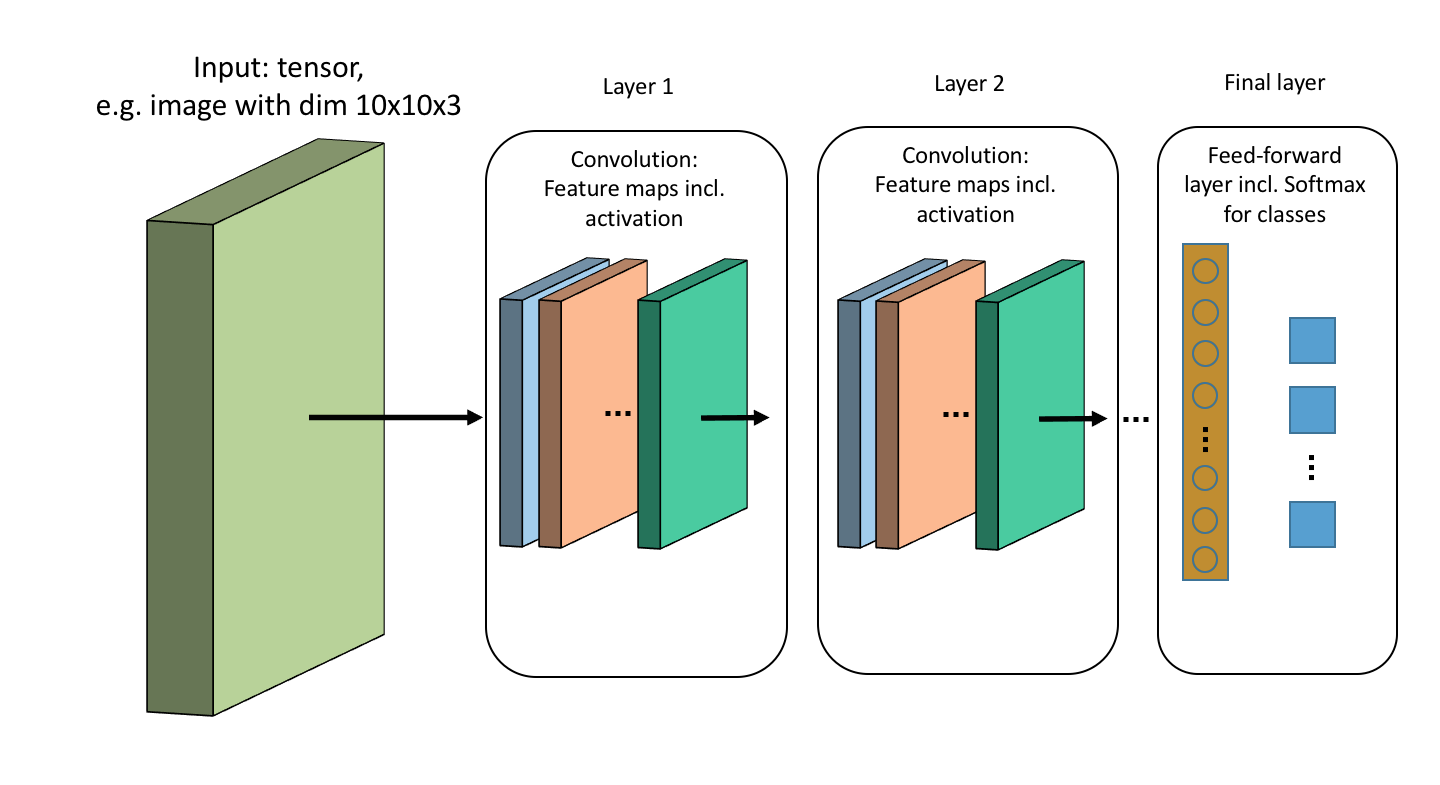
\includegraphics[width=11cm]{plots/03_first_glimpse/cnn_scheme.png}}%
        \only<1>{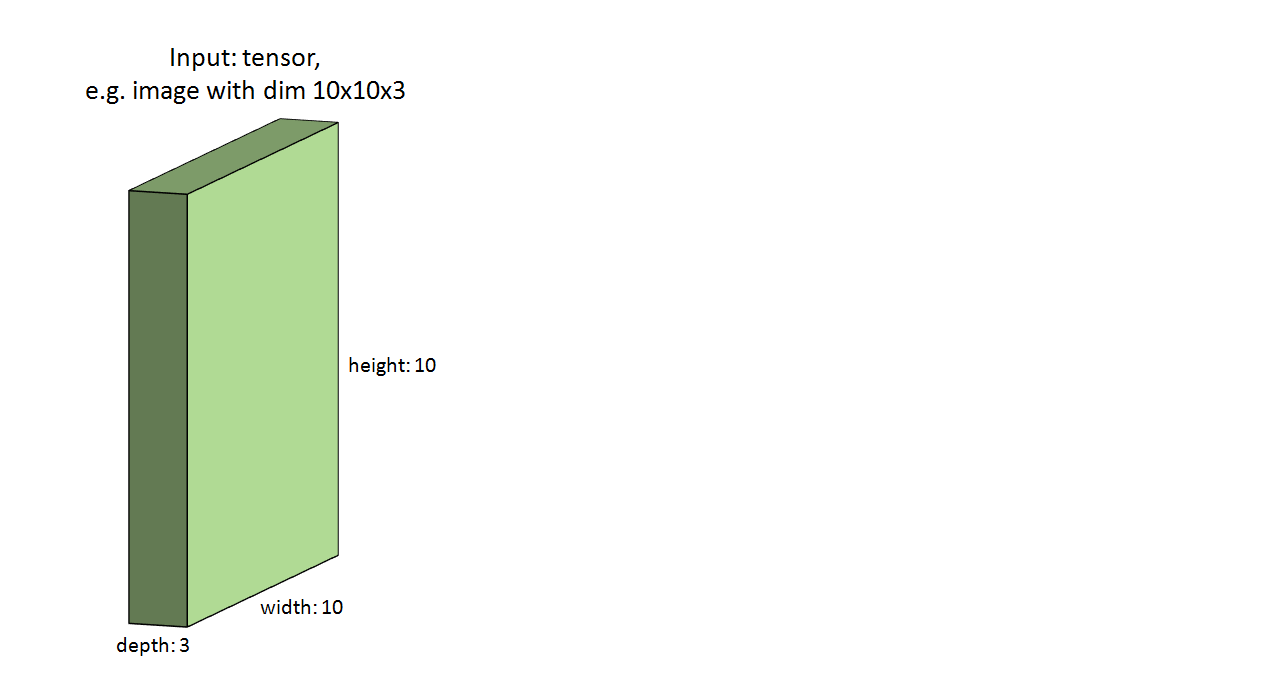
\includegraphics[width=11cm]{plots/03_first_glimpse/cnn1}}%
    \only<2>{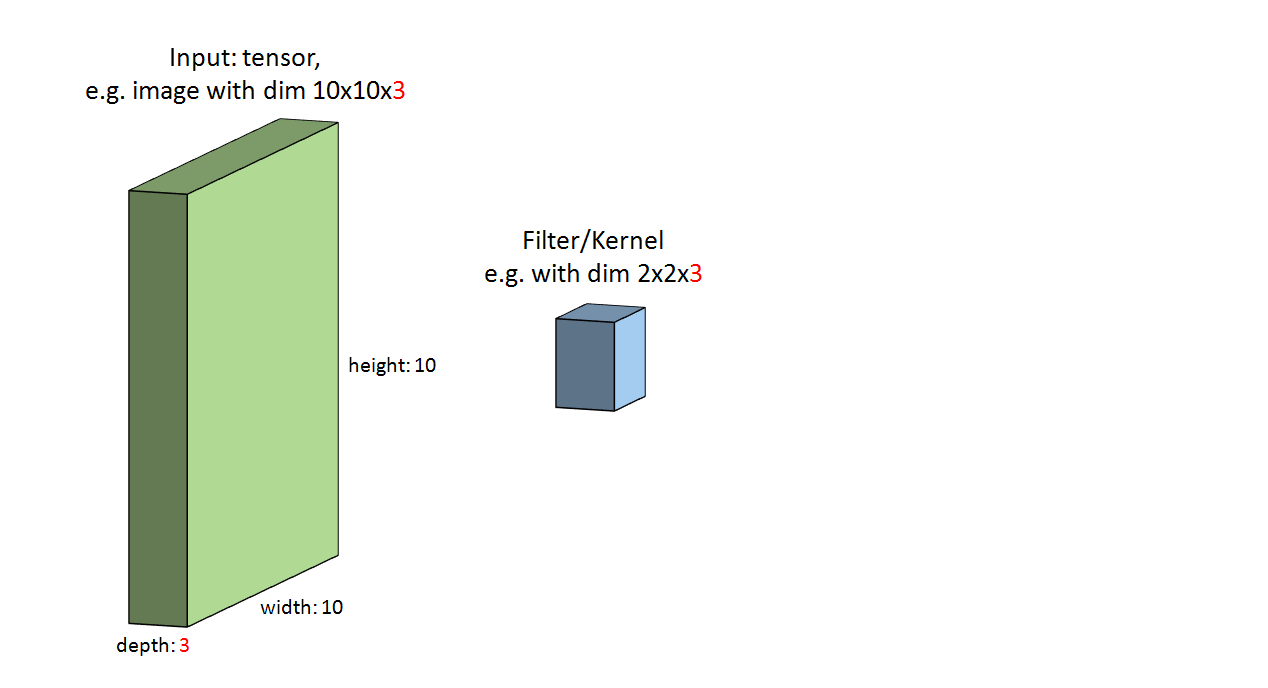
\includegraphics[width=11cm]{plots/03_first_glimpse/cnn2}}%
    \only<3>{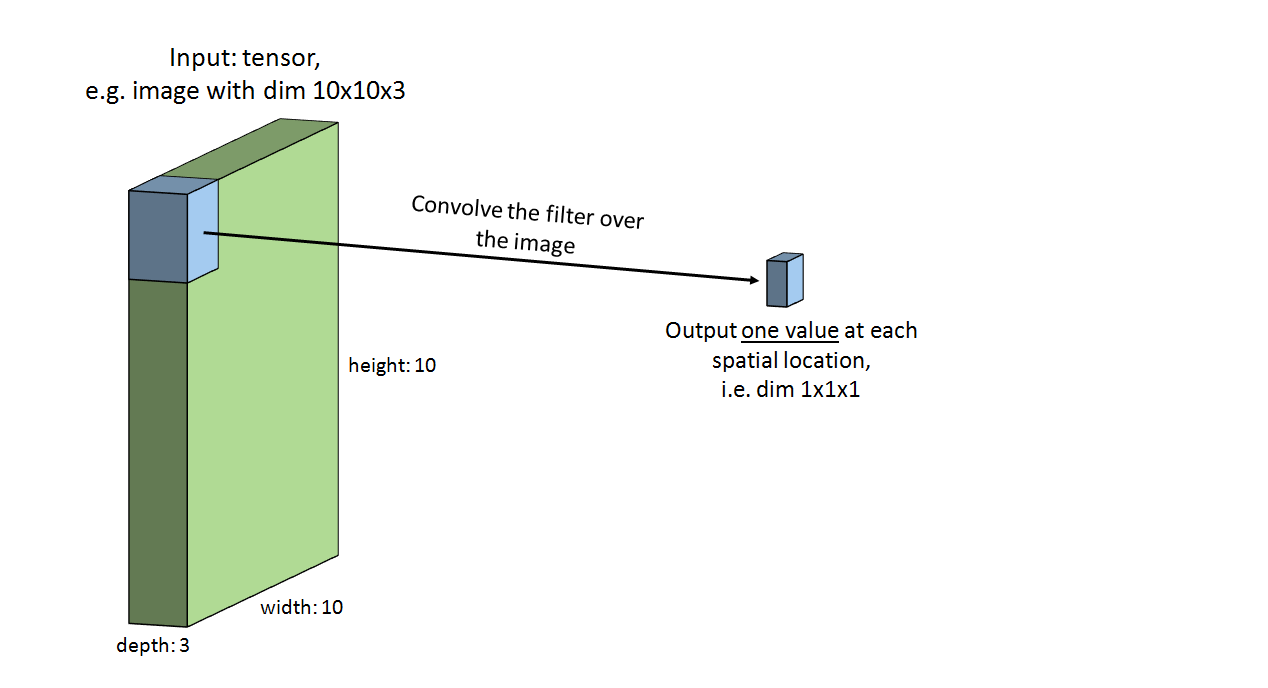
\includegraphics[width=11cm]{plots/03_first_glimpse/cnn3}}%
    \only<4>{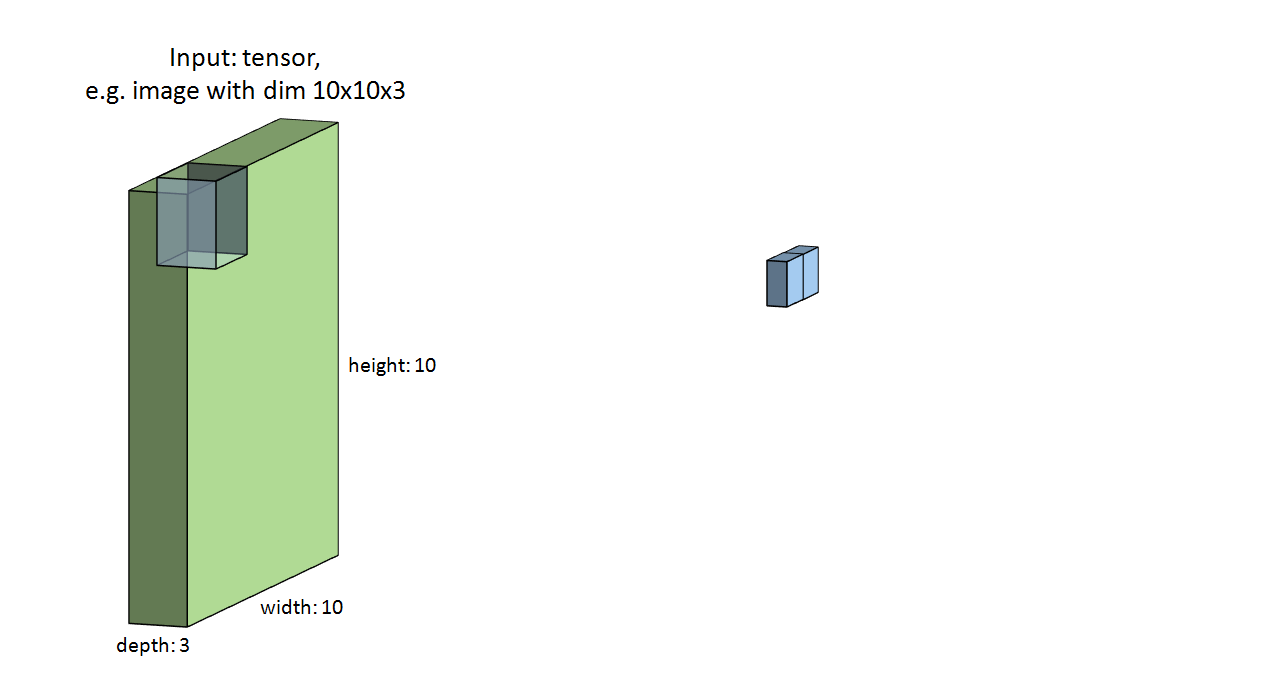
\includegraphics[width=11cm]{plots/03_first_glimpse/cnn4}}%
    \only<5>{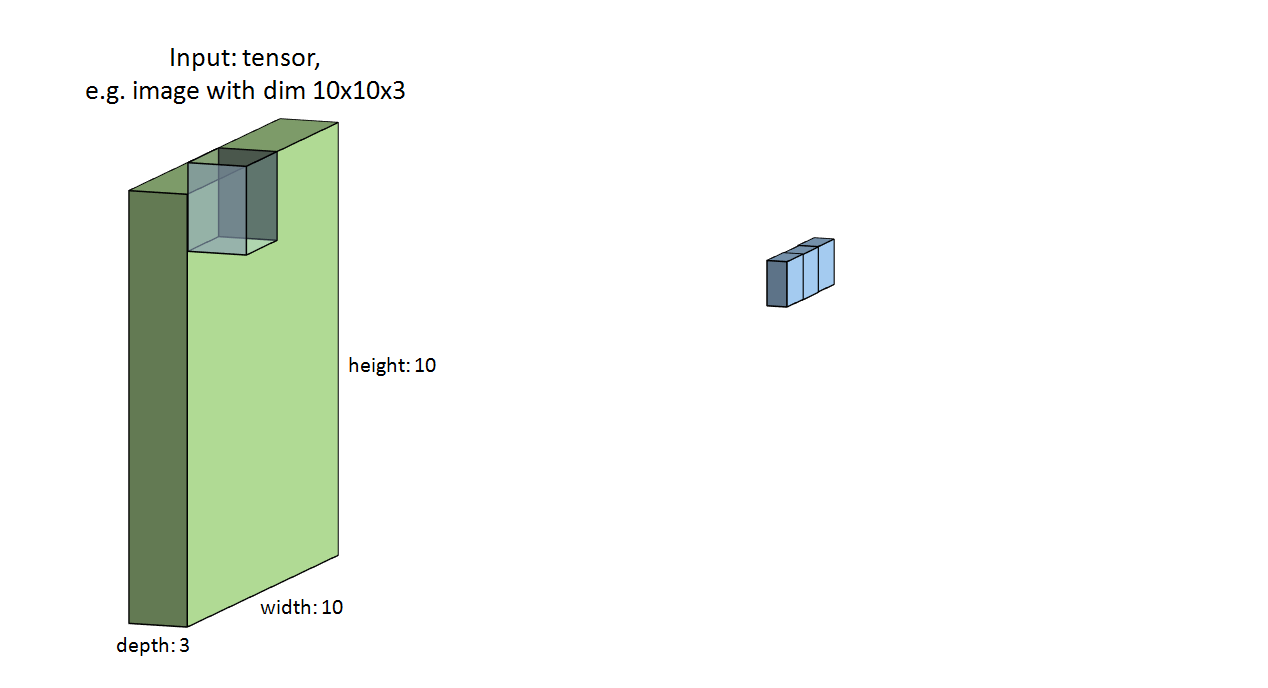
\includegraphics[width=11cm]{plots/03_first_glimpse/cnn5}}%
    \only<6>{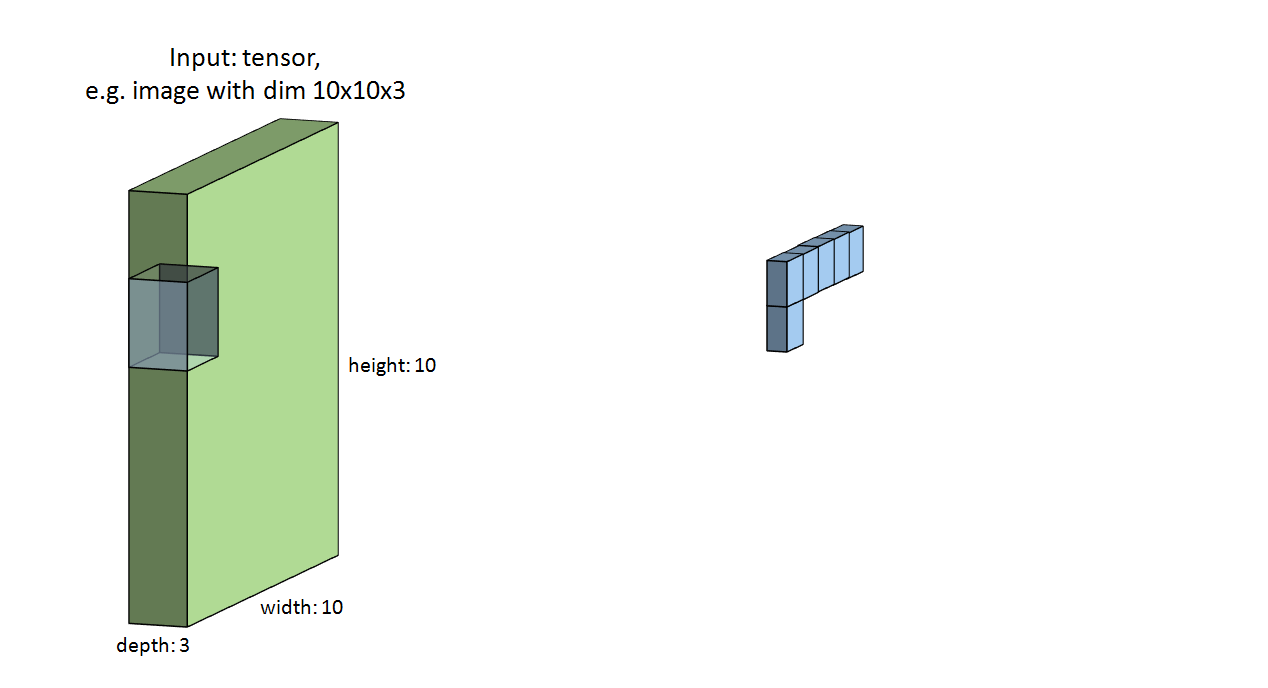
\includegraphics[width=11cm]{plots/03_first_glimpse/cnn6}}%
    \only<7>{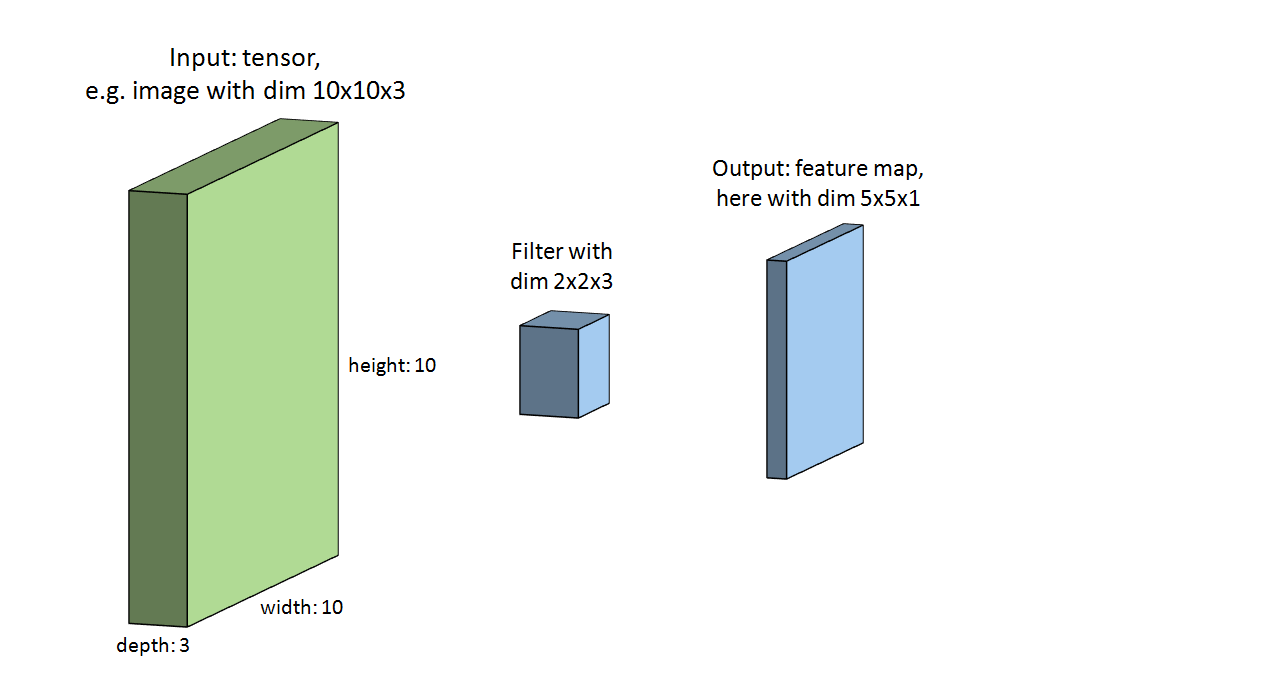
\includegraphics[width=11cm]{plots/03_first_glimpse/cnn7}}%
    \only<8>{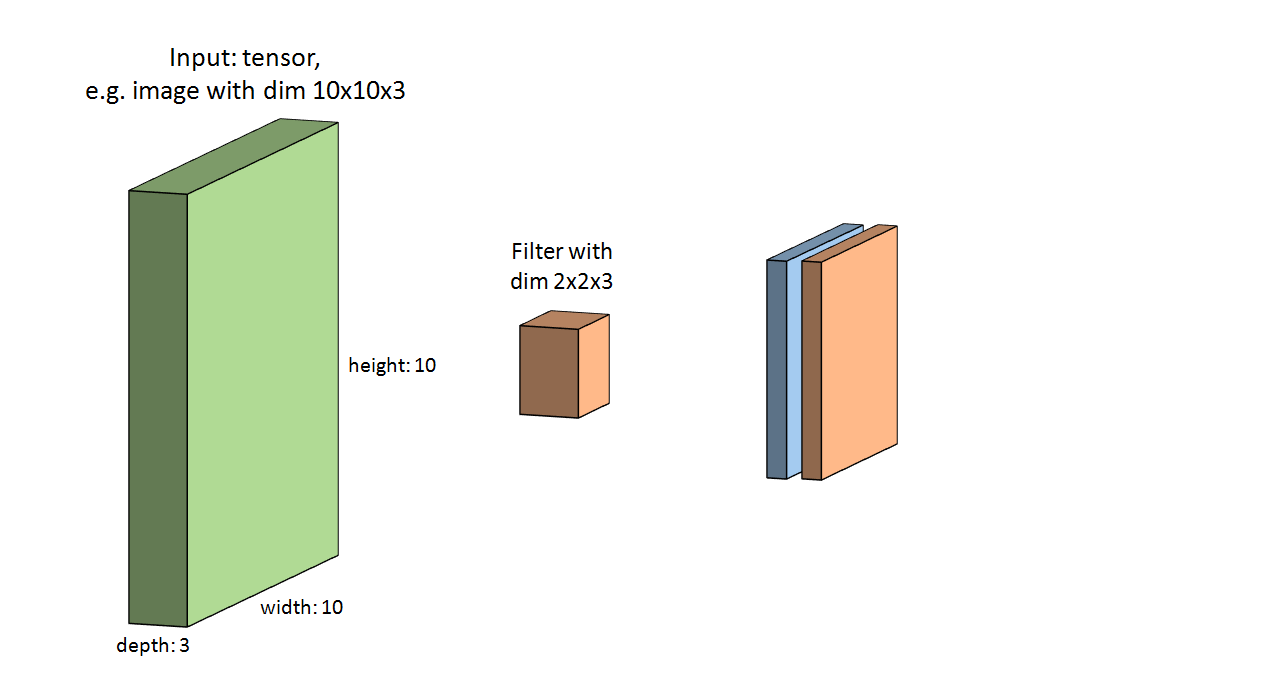
\includegraphics[width=11cm]{plots/03_first_glimpse/cnn8}}%
    \only<9>{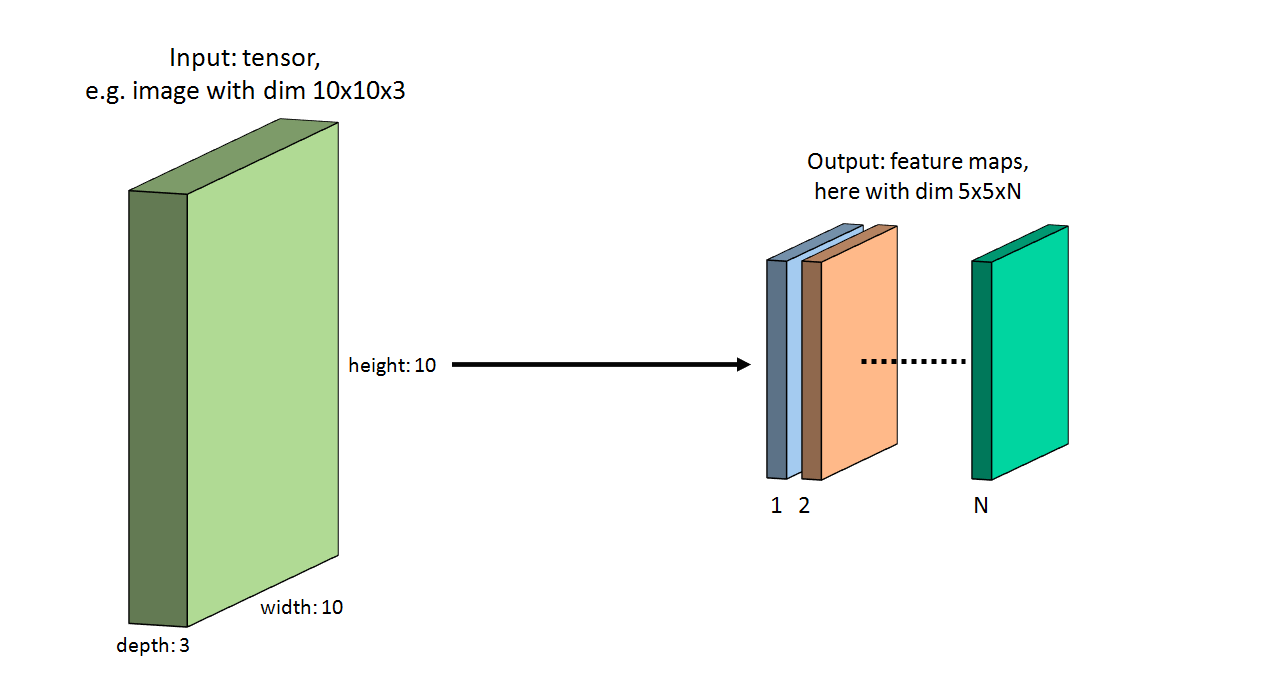
\includegraphics[width=11cm]{plots/03_first_glimpse/cnn9}}%
    \only<10>{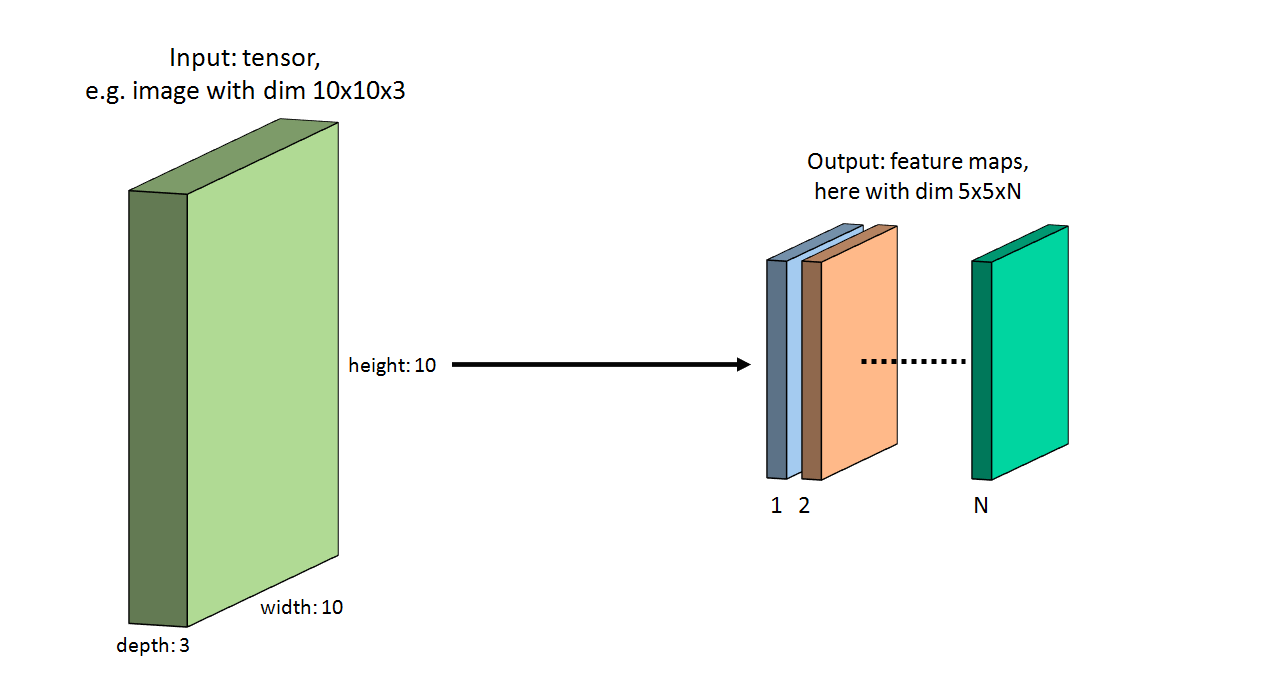
\includegraphics[width=11cm]{plots/03_first_glimpse/cnn9}}%
    \only<11>{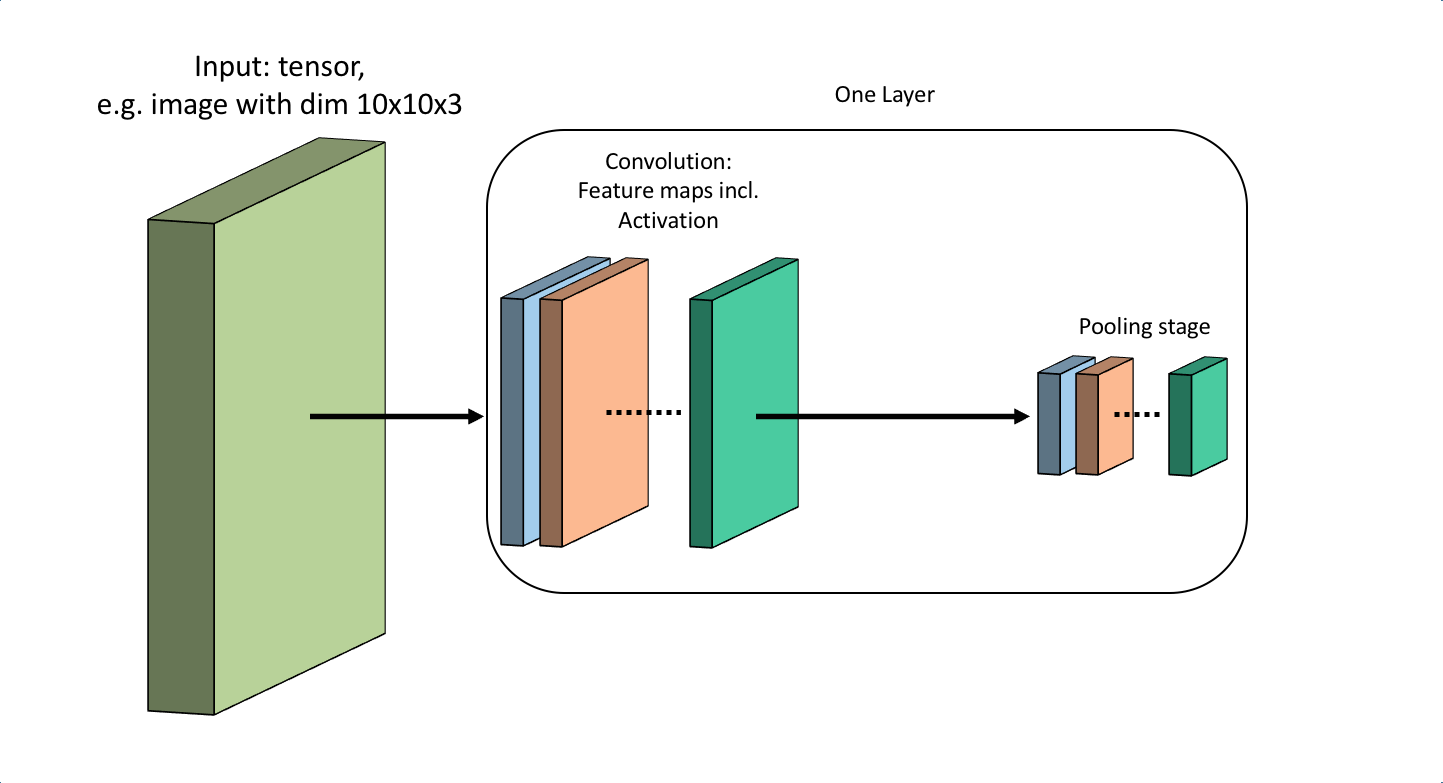
\includegraphics[width=11cm]{plots/03_first_glimpse/cnn11}}%
    \only<12>{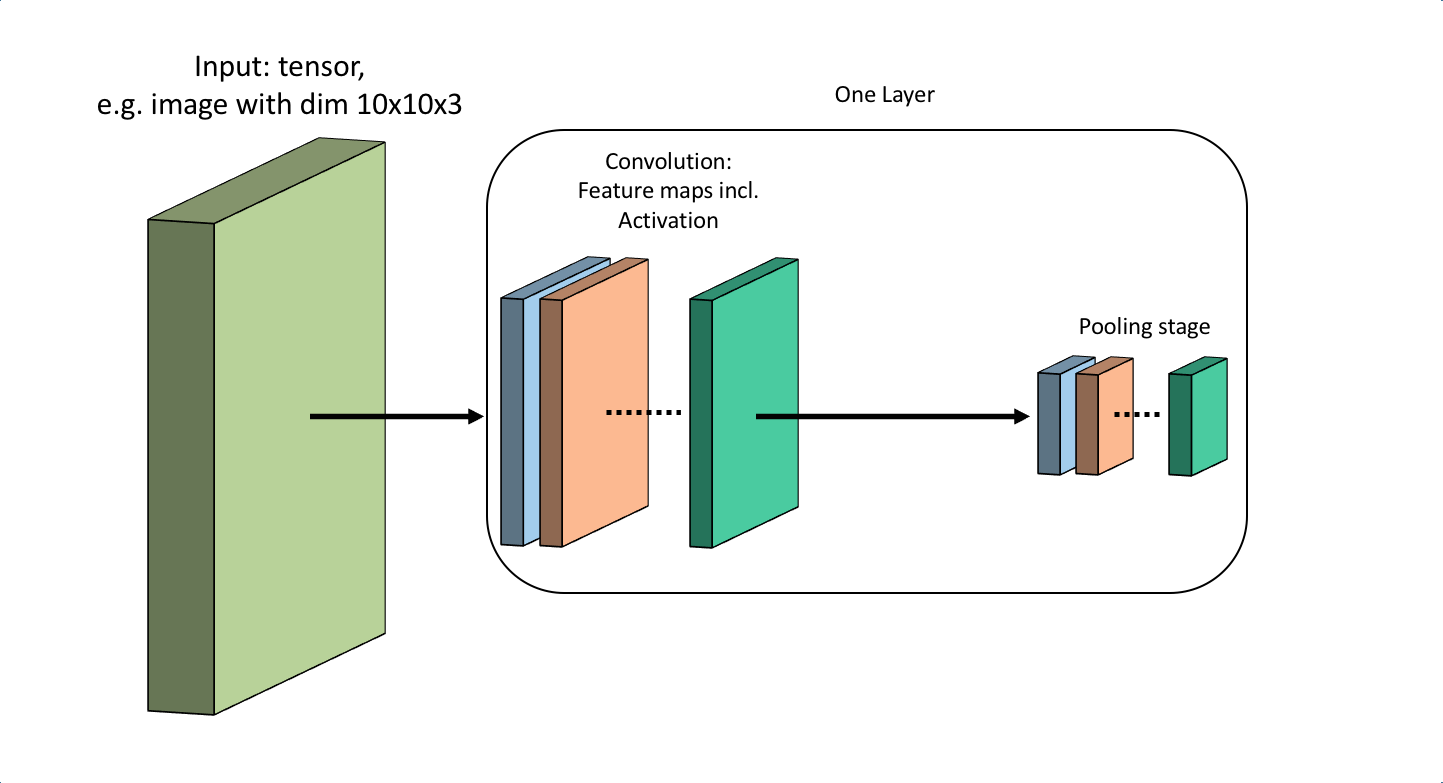
\includegraphics[width=11cm]{plots/03_first_glimpse/cnn11}}%
    \only<13>{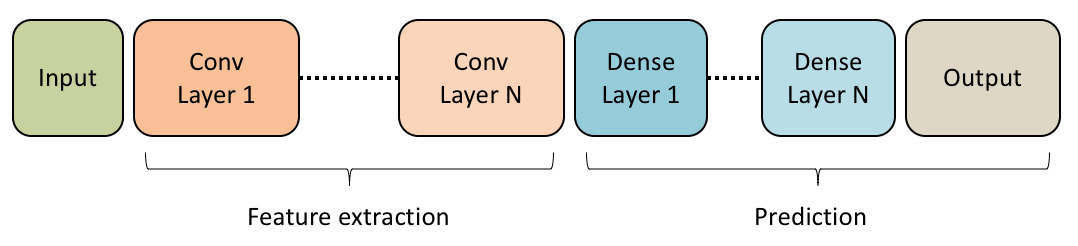
\includegraphics[width=11cm]{plots/03_first_glimpse/cnn12}}%
    
    \begin{itemize}
    %\only<1>{\item Schematic architecture of a CNN}
    \only<1>{\item Suppose we have the following input tensor with dimensions $10 \times 10 \times 3$.}
    \only<2>{\item We use a filter of size $2$.}
    \only<3>{\item Applying it to the first spatial location, yields one scalar value.}
    \only<4>{\item The second spatial location yields another one..}
    \only<5>{\item ...and another one...}
    \only<6>{\item ...and another one...}
    \only<7>{\item Finally we obtain an output which is called feature map.}
    \only<8>{\item We initialize another filter to obtain a second feature map.}
    \only<9>{\item All feature maps yield us a \enquote{new image} with dim $h \times w \times N$.}
    \only<10>{\item We actually append them to a new tensor with depth = \# filters.}
    \only<11>{\item All feature map entries will then be activated (e.g. via ReLU), just like the neurons of a standard feedforward net.}
    \only<12>{\item One may use pooling operations to downsample the dimensions of the feature maps.}
    \only<12>{\item Pooling is applied on each feature map independently: the latter, blue block is the pooled version of the previous, blue feature map.}
    \only<13>{\item Many of these layers can be placed successively, to extract even more complex features.}
    \only<13>{\item The feature maps are fed into each other sequentially. For instance, each filter from the second conv layer gets all previous feature maps from the first conv layer as an input. Each filter from the first layer extracts information from the input image tensor.}
    \only<13>{\item The feature maps of the final conv layer are flattened (into a vector) and fed into a dense layer which, in turn, is followed by more dense layers and finally, the output layer.}
    \end{itemize}
    }
    
    %%%%%%%%%%%%%%%%%%%%%%%%%%%%%%%%%%%%%%%%%%%%%%%%%%%%%%%%%%%%%%%%%%
        %%%%%%%%%%%%%%%%%%%%%%%%%%%%%%%%%%%%%%%%%%%%%%%%%%%%%%%%%%%%%%%%%%
        
        
        %%%%%%%%%%%%%%%%%%%%%%%%%%%%%%%%%%%%%%%%%%%%%%%%%%%%%%%%%%%%%%%%%%
        
        %%%%%%%%%%%%%%%%%%%%%%%%%%%%%%%%%%%%%%%%%%%%%%%%%%%%%%%%%%%%%%%%%%
        % BACKPROP NOT TREATED IN WS2018
    % TO BE DONE MORE CONCRETELY AND WITH MATH. DEPTH 
    % e.g.: https://www.jefkine.com/general/2016/09/05/backpropagation-in-convolutional-neural-networks/
        
        % \begin{vbframe}{Backpropagation}
    %   \begin{figure}
    %   \centering
    %     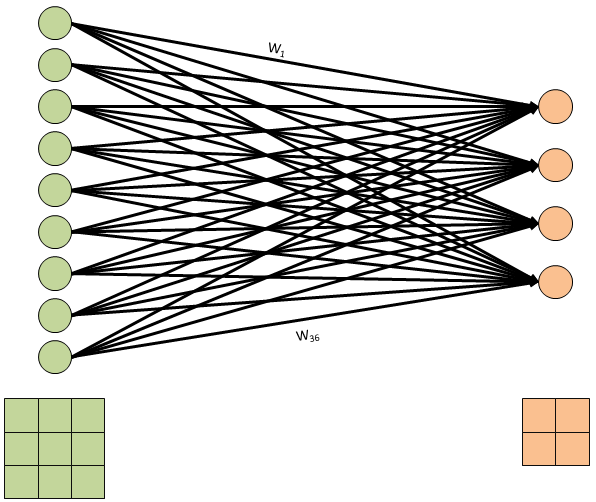
\includegraphics[width=7cm]{plots/06_conv_properties/ps/dense1.png}
    %   \end{figure}
    %   \begin{itemize}
    %     \item Assume a dense net. We had to compute 36 different gradients to adjust our network (36 weights).
    %   \end{itemize}
    % \end{vbframe}
    % 
    % \frame{
        % \frametitle{Backpropagation}
        % 
        %   \center
        %   \only<1>{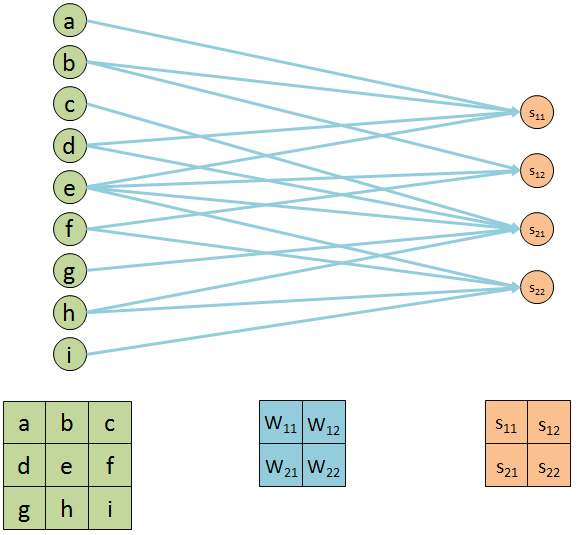
\includegraphics[width=6.5cm]{plots/09_backprop/bp1.png}}%
            %   \only<2>{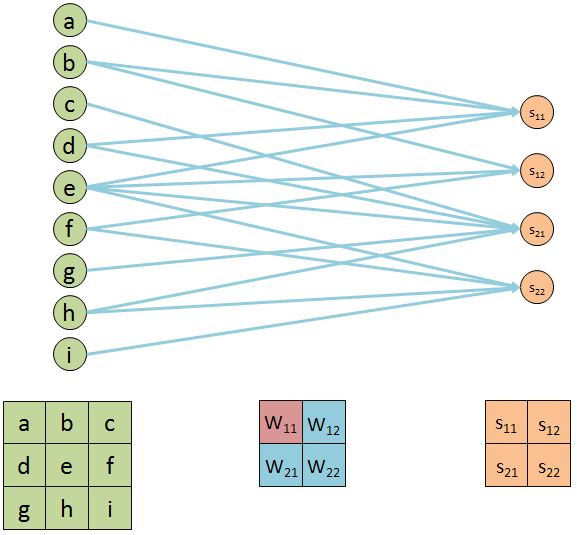
\includegraphics[width=6.5cm]{plots/09_backprop/bp2.png}}%
            %   \only<3>{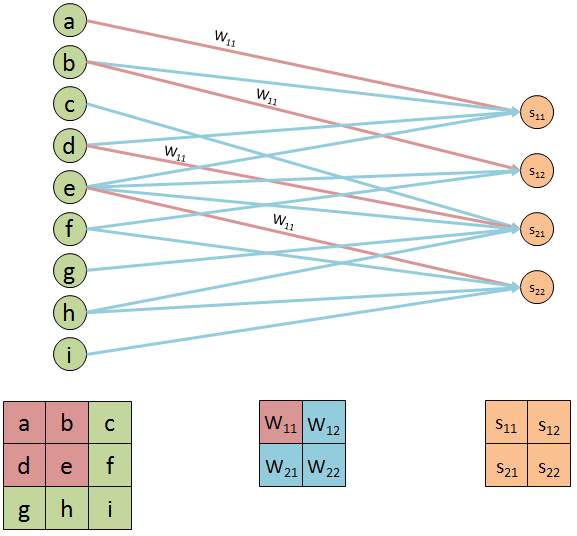
\includegraphics[width=6.5cm]{plots/09_backprop/bp4.png}}%
            % 
        %   \begin{itemize}
        % 
        %     \only<1>{\item We've already learned that our CNN only has 4 weights.}
%     \only<2>{\item Let us focus once again on weight $w_{11}$}
%     \only<3>{\item The highlited connections shows where $w_{11}$ incorporates.}
% 
%   \end{itemize}
% }
% 
% \frame{
% \frametitle{Backpropagation}
% 
%   \begin{itemize}
% 
%     \only<1-5>{\item We know from earlier computations:}
%     \only<1-2>{\item[] $s_{11} = a \cdot w_{11} + b \cdot w_{12} + d \cdot w_{21} + e \cdot w_{22}$}
%     \only<1-2>{\item[] $s_{12} = b \cdot w_{11} + c \cdot w_{12} + e \cdot w_{21} + f \cdot w_{22}$}
%     \only<1-2>{\item[] $s_{21} = d \cdot w_{11} + e \cdot w_{12} + g \cdot w_{21} + h \cdot w_{22}$}
%     \only<1-2>{\item[] $s_{22} = e \cdot w_{11} + f \cdot w_{12} + h \cdot w_{21} + i \cdot w_{22}$}
%     \only<3-4>{\item[] $s_{11} = a \cdot \textcolor{red}{w_{11}} + b \cdot w_{12} + d \cdot w_{21} + e \cdot w_{22}$}
%     \only<3-4>{\item[] $s_{12} = b \cdot \textcolor{red}{w_{11}} + c \cdot w_{12} + e \cdot w_{21} + f \cdot w_{22}$}
%     \only<3-4>{\item[] $s_{21} = d \cdot \textcolor{red}{w_{11}} + e \cdot w_{12} + g \cdot w_{21} + h \cdot w_{22}$}
%     \only<3-4>{\item[] $s_{22} = e \cdot \textcolor{red}{w_{11}} + f \cdot w_{12} + h \cdot w_{21} + i \cdot w_{22}$}
%     \only<5>{\item[] $s_{11} = \textcolor{red}{a} \cdot w_{11} + b \cdot w_{12} + d \cdot w_{21} + e \cdot w_{22}$}
%     \only<5>{\item[] $s_{12} = \textcolor{red}{b} \cdot w_{11} + c \cdot w_{12} + e \cdot w_{21} + f \cdot w_{22}$}
%     \only<5>{\item[] $s_{21} = \textcolor{red}{d} \cdot w_{11} + e \cdot w_{12} + g \cdot w_{21} + h \cdot w_{22}$}
%     \only<5>{\item[] $s_{22} = \textcolor{red}{e} \cdot w_{11} + f \cdot w_{12} + h \cdot w_{21} + i \cdot w_{22}$}
%     \only<1-5>{\item[]}
%     \only<2-5>{\item To obtain gradients for our weights, we simply compute:}
%     \only<1-5>{\item[]}
%     \only<2>{\item
%       $\frac{\delta s_{i,j}}{\delta w}$ = $\begin{pmatrix} 
%       \sum\limits_{i} \sum\limits_{j} \frac{\delta s_{ij}}{\delta w_{11}} & 
%       \sum\limits_{i} \sum\limits_{j} \frac{\delta s_{ij}}{\delta w_{12}} \\ 
%       \sum\limits_{i} \sum\limits_{j} \frac{\delta s_{ij}}{\delta w_{21}} & 
%       \sum\limits_{i} \sum\limits_{j} \frac{\delta s_{ij}}{\delta w_{22}}
%       \end{pmatrix}$    
%     }
%     \only<3>{\item
%       $\frac{\delta s_{i,j}}{\delta w}$ = $\begin{pmatrix} 
%       \sum\limits_{i} \sum\limits_{j} \frac{\delta s_{ij}}{\delta \textcolor{red}{w_{11}}} & 
%       \sum\limits_{i} \sum\limits_{j} \frac{\delta s_{ij}}{\delta w_{12}} \\ 
%       \sum\limits_{i} \sum\limits_{j} \frac{\delta s_{ij}}{\delta w_{21}} & 
%       \sum\limits_{i} \sum\limits_{j} \frac{\delta s_{ij}}{\delta w_{22}}
%       \end{pmatrix}$    
%     }
%     \only<4>{\item 
%       $\frac{\delta s_{i,j}}{\delta w}$ = $\begin{pmatrix} 
%       \frac{\delta s_{11}}{\delta \textcolor{red}{w_{11}}} + 
%       \frac{\delta s_{12}}{\delta \textcolor{red}{w_{11}}} + 
%       \frac{\delta s_{21}}{\delta \textcolor{red}{w_{11}}} + 
%       \frac{\delta s_{22}}{\delta \textcolor{red}{w_{11}}} & &
%       .... \\
%       \textcolor{white}{bla} \\
%       .... & &
%       ....
%       \end{pmatrix}$
%     }
%     \only<5>{\item
%       $\frac{\delta s_{i,j}}{\delta w}$ = $\begin{pmatrix} 
%       \textcolor{red}{a} + \textcolor{red}{b} + \textcolor{red}{d} + \textcolor{red}{e} & &
%       b + c + e + f \\
%       \textcolor{white}{bla} \\
%       d + e + g + h & &
%       e + f + h + i
%       \end{pmatrix}$    
%     }
%   \end{itemize}
% }

%%%%%%%%%%%%%%%%%%%%%%%%%%%%%%%%%%%%%%%%%%%%%%%%%%%%%%%%%%%%%%%%%%
%%%%%%%%%%%%%%%%%%%%%%%%%%%%%%%%%%%%%%%%%%%%%%%%%%%%%%%%%%%%%%%%%%
% \begin{vbframe}{Convolution mathematically - content}
%     \begin{itemize}
%         \item Sources:
%         \item nice explanation here: https://wiki.tum.de/display/lfdv/Convolutional+Neural+Networks
%         \item and here: https://wiki.tum.de/display/lfdv/Layers+of+a+Convolutional+Neural+Network
%         \item and dl book: http://www.deeplearningbook.org/contents/convnets.html
%         \item cornell uni: google cornell cs1114 convolution
%     \end{itemize}
% \end{vbframe}    


%%%%%%%%%%%%%%%%%%%%%%%%%%%%%%%%%%%%%%%%%%%%%%%%%%%%%%%%%%%%%%%%%%
\section{Applications}
%%%%%%%%%%%%%%%%%%%%%%%%%%%%%%%%%%%%%%%%%%%%%%%%%%%%%%%%%%%%%%%%%%
\begin{vbframe}{Application - Image Classification}
    \begin{itemize}
        \item One of use case for CNNs is image classification.
        \item There exist a broad variety of battle-proven image classification architecture such as the AlexNet , the Inception Net or the ResNet which will be discussed in detail in the next lecture.
        \item All those architectures rely on a set of subsequent convolutional filters and aim to learn the mapping from an image to a probability score over a set of classes.
    \end{itemize}
\framebreak
    \begin{figure}
        \centering
        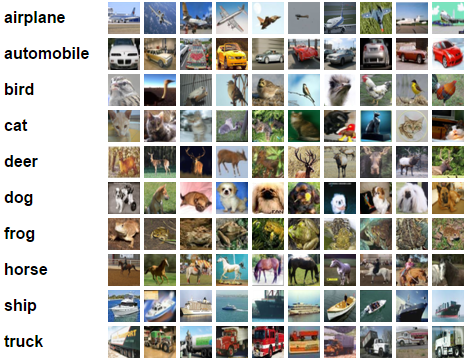
\includegraphics[width=7cm]{plots/01_introduction/recognition.png}
        \caption{Image classification with Cifar 10: famous benchmark dataset with 60000 images and 10 classes (Alex Krizhevsky (2009)). There is also a much more difficult version with 60000 images and 100 classes.}
    \end{figure}
\framebreak
    \begin{figure}
        \centering
        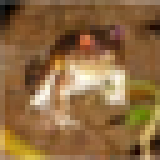
\includegraphics[width=4cm]{plots/application/cifar_frog.png}
        \caption{One example of the Cifar10 data: A highly pixelated, coloured image of a frog with dimension [32, 32, 3]. }
    \end{figure}
\framebreak
    \begin{figure}
        \centering
          \scalebox{1}{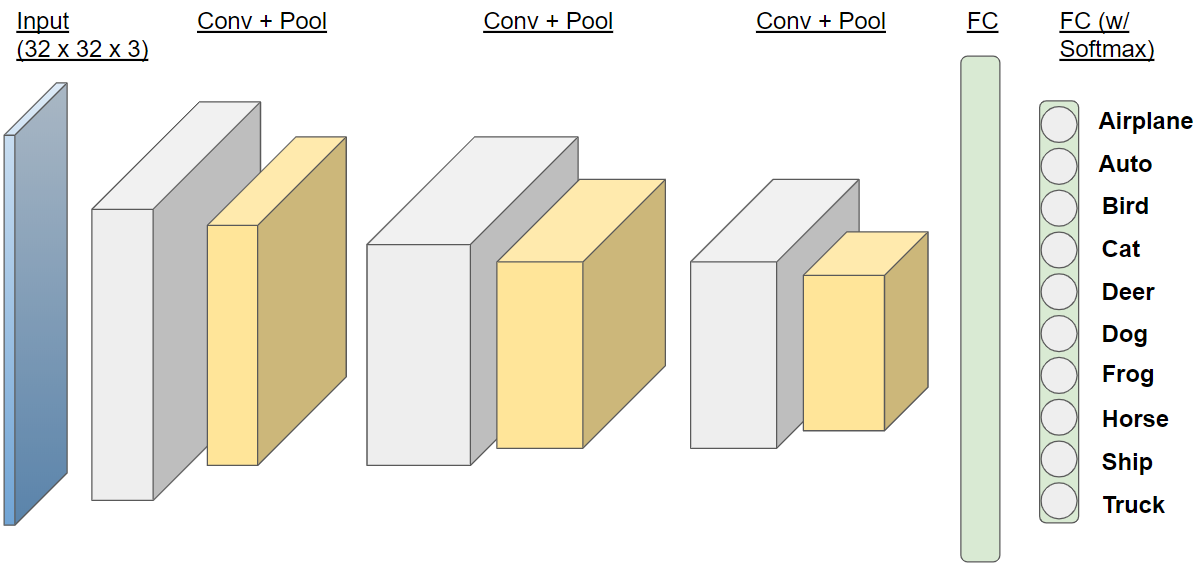
\includegraphics{plots/application/cifar10_eg.png}}
        \caption{An example of a CNN architecture for classification on the Cifar10 dataset (FC = Fully Connected). }
    \end{figure}  
\end{vbframe}

\begin{frame} {CNN vs a Fully Connected net on Cifar10}
  \begin{figure}
        \centering
          \scalebox{0.75}{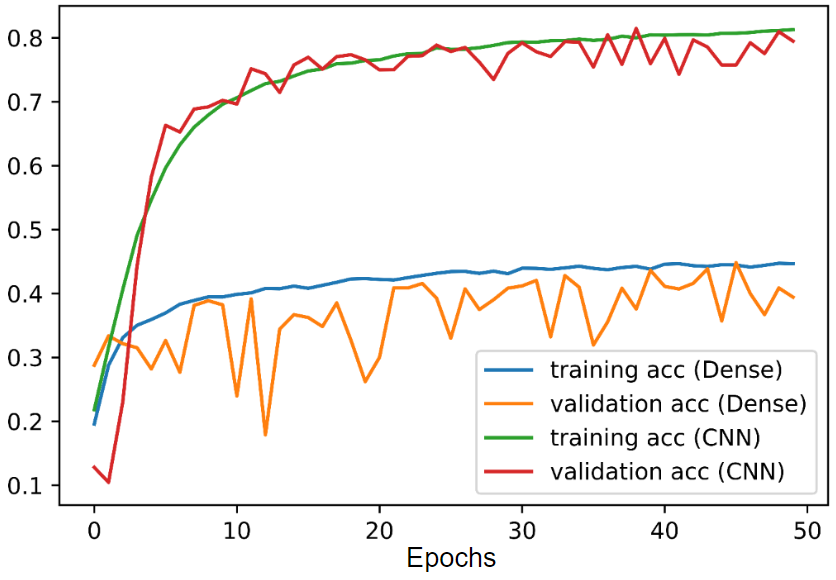
\includegraphics{plots/application/cnn_vs_dense_1.png}}
        \caption{Performance of a CNN and a fully connected neural net ("Dense") on Cifar-10. Both networks have roughly the same number of layers. They were trained using the same learning rate, weight decay and dropout rate. Of course, the CNN performs better because it has less learnable parameters and the right inductive bias for the task.}
    \end{figure} 
\end{frame}
%%%%%%%%%%%%%%%%%%%%%%%%%%%%%%%%%%%%%%%%%%%%%%%%%%%%%%%%%%%%%%%%%%
%%%%%%%%%%%%%%%%%%%%%%%%%%%%%%%%%%%%%%%%%%%%%%%%%%%%%%%%%%%%%%%%%%
\begin{vbframe}{Application - Image Colorization}
    \begin{itemize}
        \item Basic idea (introduced by Zhang et al., 2016):
        \begin{itemize}
            \item Train the net on pairs of grayscale and coloured images.
            \item Force it to make a prediction on the colour-value \textbf{for each pixel} in the grayscale input image.
            \item Combine the grayscale-input with the colour-output to yield a colorized image.
        \end{itemize}
        \item Very comprehensive material on the method is provided on the author's website. \href{http://richzhang.github.io/colorization/}{\beamergotobutton{Click here}}
            \end{itemize}
            \framebreak
            \begin{figure}
            \centering
            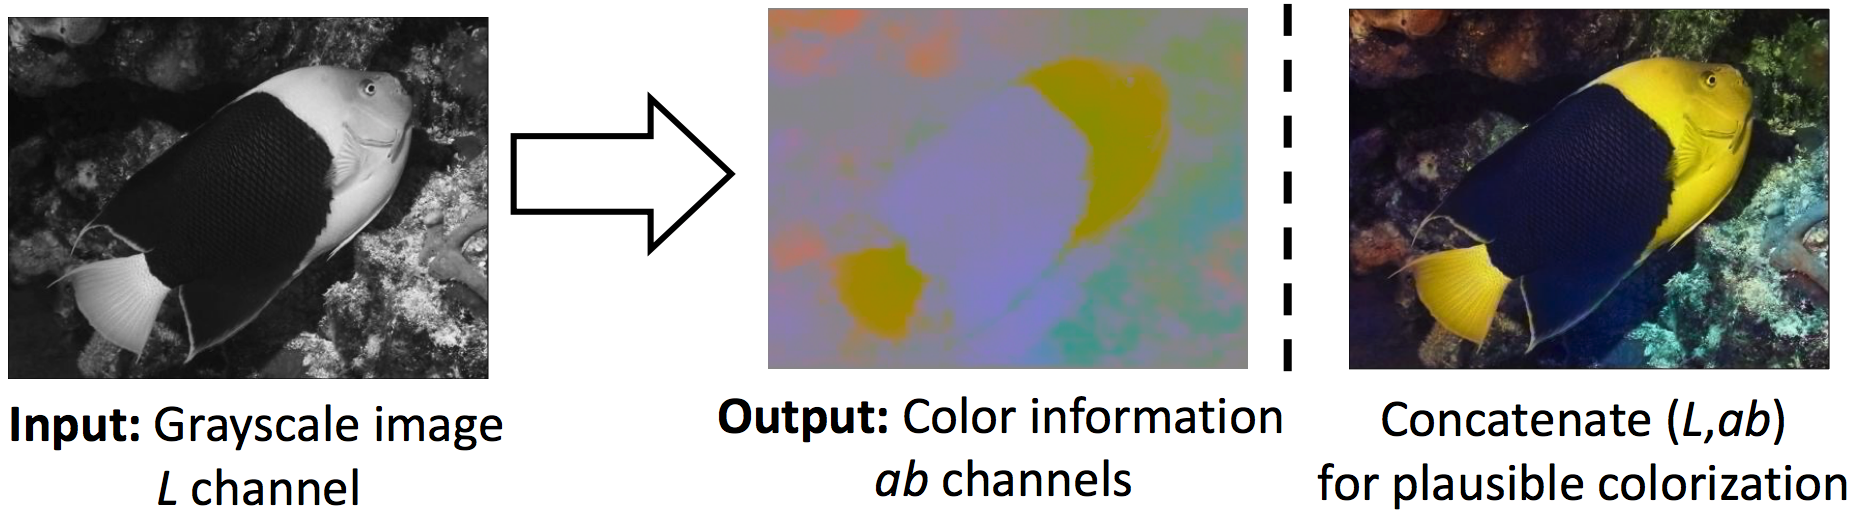
\includegraphics[width=11cm]{plots/application/fish_lab.png}
            \caption{The CNN learns the mapping from grayscale (L) to color (ab) for each pixel in the image. The L and ab maps are then concatenated to yield the colorized image. The authors use the LAB color space for the image representation.}
            \end{figure}
            \framebreak
            \begin{figure}
            \centering
            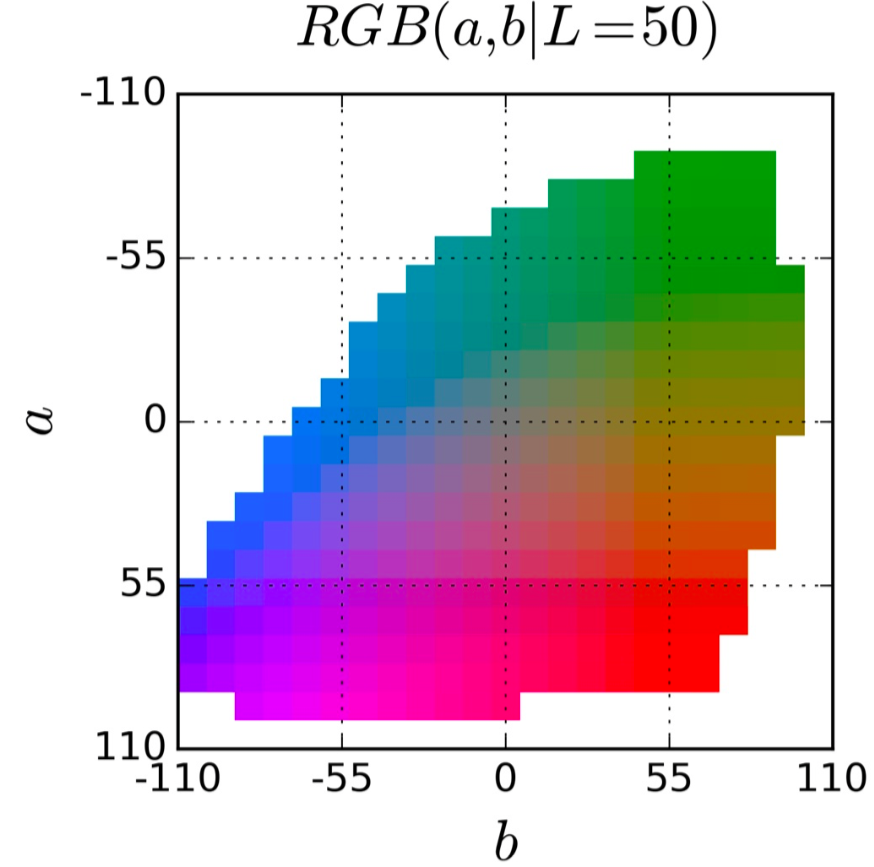
\includegraphics[width=5cm]{plots/application/lab.png}
            \caption{The colour space (ab) is quantized in a total of 313 bins. This allows to treat the color prediction as a classification problem where each pixel is assigned a probability distribution over the 313 bins and that with the highest softmax-score is taken as predicted color value. The bin is then mapped back to the corresponding, numeric (a,b) values. The network is optimized using a multinomial cross entropy loss over the 313 quantized (a,b) bins.}
            \end{figure}
            \framebreak
            \begin{figure}
            \centering
            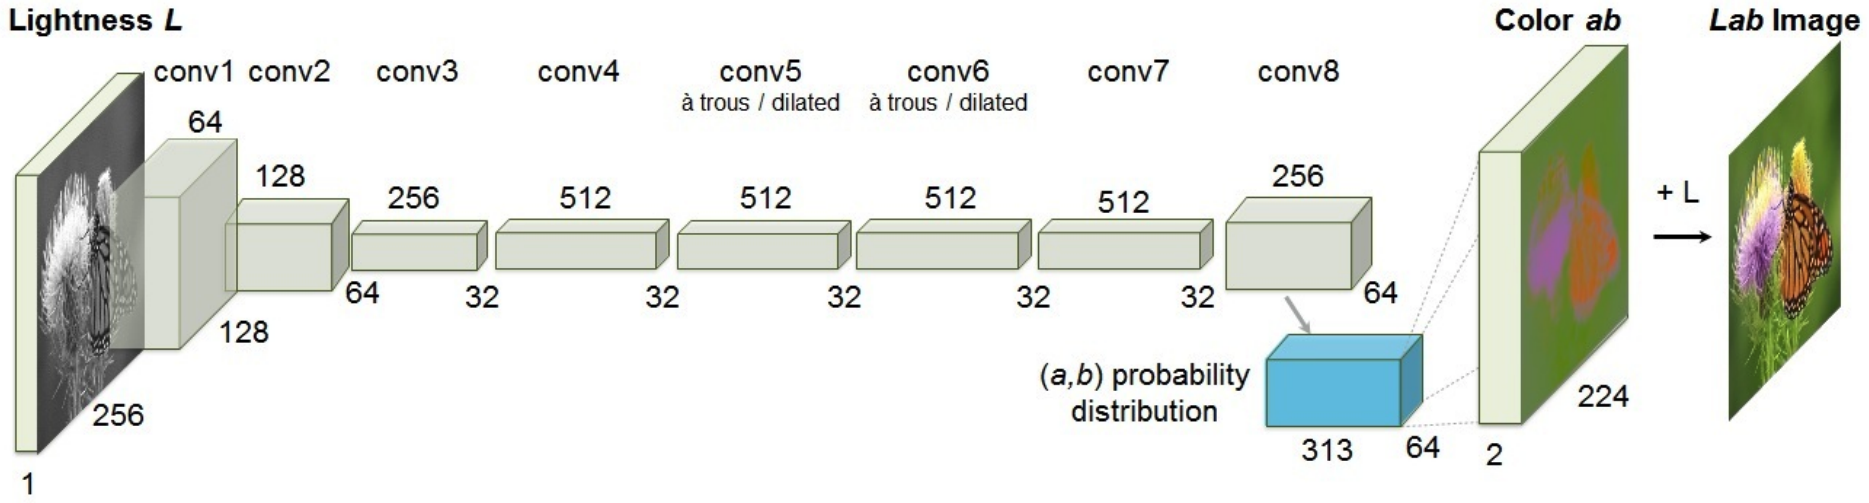
\includegraphics[width=11.5cm]{plots/application/color_architecture.png}
            \caption{The architecture consists of stacked CNN layers which are upsampled towards the end of the net. It makes use of \textit{dilated convolutions} and \textit{upsampling layers} which are explained in the next lecture. The output is a tensor of dimension [64, 64, 313] that stores the 313 probabilities for each element of the final, downsampled 64x64 feature maps.} 
            \end{figure}
            \framebreak
            \begin{figure}
            \centering
            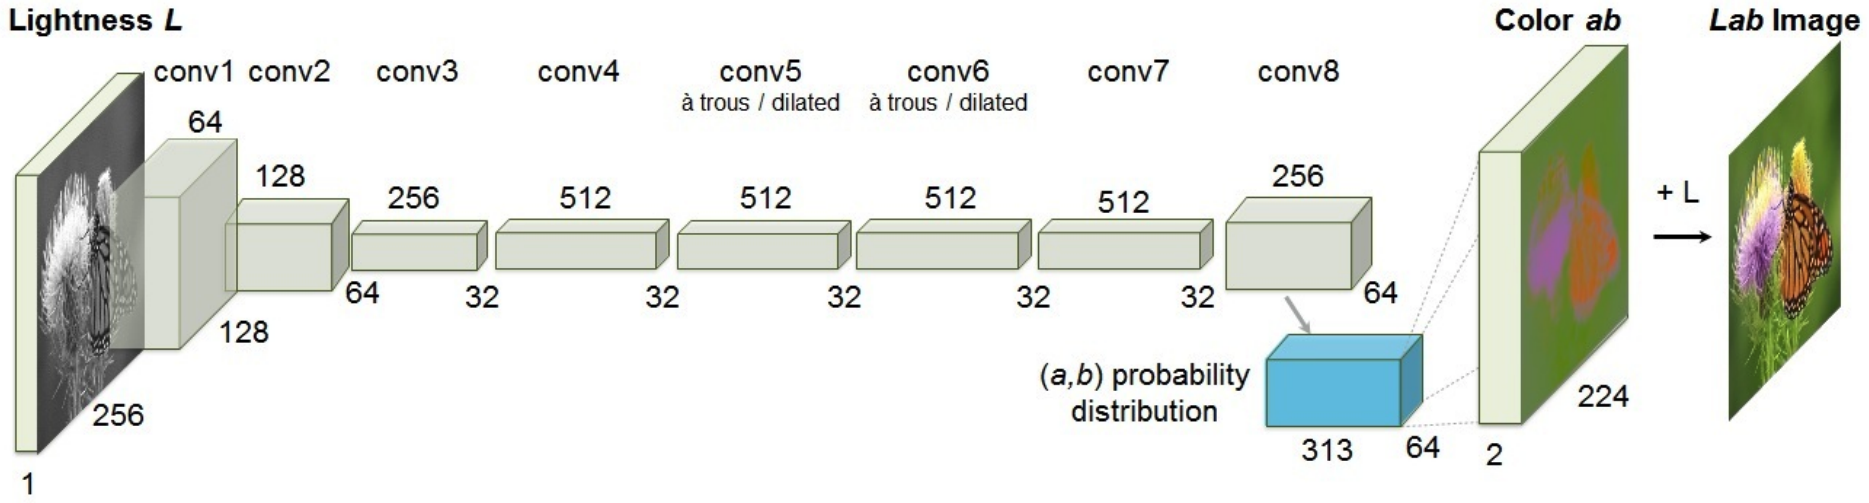
\includegraphics[width=11.5cm]{plots/application/color_architecture.png}
            \caption{This block is then upsampled to a dimension of 224x224 and the predicted color bins are mapped back to the (a,b) values yielding a depth of 2. Finally, the L and the ab maps are concatenated to yield a colored image.} 
            \end{figure}
            \end{vbframe}
            %%%%%%%%%%%%%%%%%%%%%%%%%%%%%%%%%%%%%%%%%%%%%%%%%%%%%%%%%%%%%%%%%%
                %%%%%%%%%%%%%%%%%%%%%%%%%%%%%%%%%%%%%%%%%%%%%%%%%%%%%%%%%%%%%%%%%%
                \begin{vbframe}{Application - Object localization}
            \begin{itemize}
            \item Until now, we used CNNs for \textit{single}-class classification of images - \textbf{which object is on the image?}
            \item Now we extend this framework - \textbf{is there an object in the image and if yes, where and which?}
            \end{itemize}
            \begin{figure}
            \centering
            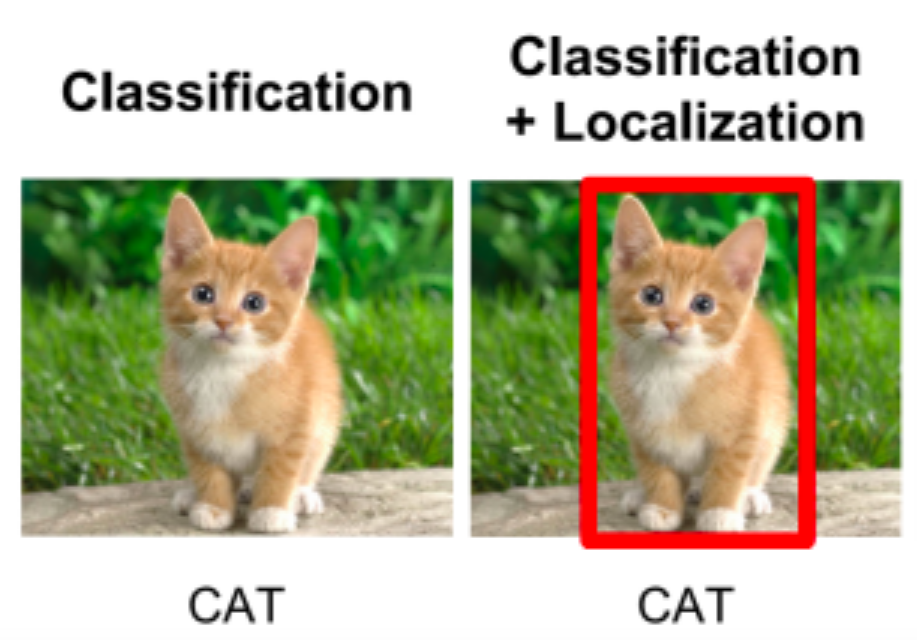
\includegraphics[width=4cm]{plots/application/localize_cat.png}
            \caption{Classify and detect the location of the cat.}
            \end{figure}
            \framebreak
            \begin{itemize}
            % source1:  https://medium.com/machine-learning-bites/deeplearning-series-objection-detection-and-localization-yolo-algorithm-r-cnn-71d4dfd07d5f
            % source2: https://leonardoaraujosantos.gitbooks.io/artificial-inteligence/content/object_localization_and_detection.html
            \item Bounding boxes can be defined by the location of the left lower corner as well as the height and width of the box: [$b_x$, $b_y$, $b_h$, $b_w$].
            \item We now combine three tasks (detection, classification and localization) in one architecture.
            \item This can be done by adjusting the label output of the net.
            \item Imagine a task with three classes (cat, car, frog).
            \item In standard classification we would have: 
                $$
                \text{label vector}
            \begin{bmatrix}
            c_{cat}\\
            c_{car} \\
            c_{frog}
            \end{bmatrix}
            \text{and softmax output}
            \begin{bmatrix}
            P(y = cat| X, \theta)\\
            P(y = car| X, \theta)\\
            P(y = frog| X, \theta)
            \end{bmatrix}
            $$
                \end{itemize}
            \framebreak
            \begin{itemize}
            \item We include the information, if there is a object as well as the bounding box parametrization in the label vector.
            \item This gives us the following label vector:
                $$
                \begin{bmatrix}
            b_x\\
            b_y \\
            b_h \\
            b_w \\
            c_o \\
            c_{cat} \\
            c_{car} \\
            c_{frog} \\
            \end{bmatrix} =             
                \begin{bmatrix}
            \text{x coordinate box}\\
            \text{y coordinate box} \\
            \text{height box} \\
            \text{width box} \\
            \text{presence of object, binary} \\
            \text{class cat, one-hot} \\
            \text{class car, one-hot}\\
            \text{class frog, one-hot} \\
            \end{bmatrix}
            $$
                \end{itemize}
            \framebreak
            \begin{figure}
            \centering
            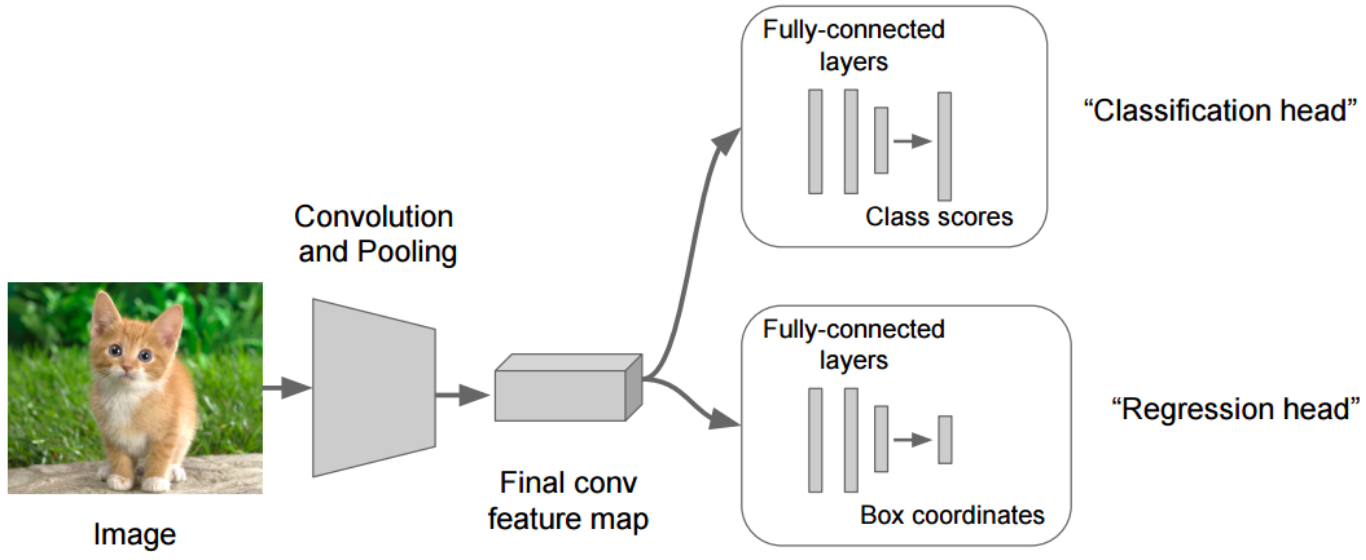
\includegraphics[width=8cm]{plots/application/naive_localization.png}
            \end{figure}
            \begin{itemize}
            \item Naive approach: use a CNN with two heads, one for the class classification and one for the bounding box regression.
            \item But: What happens, if there are two cats in the image?
                \item Different approaches: "Region-based" CNNs (R-CNN, Fast R-CNN and Faster R-CNN) and "single-shot" CNNs (SSD and YOLO).
            \end{itemize}
            % \framebreak
            %     \begin{itemize}
            %         \item \textbf{Q to reviewers: go on or too much? Would require +5 slides to explain Faster RCNN in a rough manner}
            %         \item plenty of good resources out there:
                %         \item \href{https://leonardoaraujosantos.gitbooks.io/artificial-inteligence/content/object_localization_and_detection.html}{1}
            %         \item \href{https://blog.athelas.com/a-brief-history-of-cnns-in-image-segmentation-from-r-cnn-to-mask-r-cnn-34ea83205de4}{2}
            %         \item \href{https://towardsdatascience.com/r-cnn-fast-r-cnn-faster-r-cnn-yolo-object-detection-algorithms-36d53571365e}{3}
            %         \item \href{http://www.robots.ox.ac.uk/~tvg/publications/talks/fast-rcnn-slides.pdf}{4}
            %     \end{itemize}
            \end{vbframe}
            
            
            
            
            
            
            
            
            
            % \begin{vbframe}{Convolution mathematically - 2D}
            %     \begin{itemize}
            %         \item Interpret images as data matrices
            %         \item Amount of channels determines amount of matrices (RGB: 3, BW: 1)
            %         \item One channel of image $\mathcal{I}$ is represented as a matrix:\\
            %             \begin{equation*}
            %                 \begin{split}
            %                 \mathcal{I}:\Omega \in \R^2 &\mapsto \R_+ \\
            %                 (i, j) \mapsto \mathcal{I}_{i, j}
            %                 \end{split}
            %             \end{equation*}
            %         \item $\mathcal{I}$ contains two axis $\rightarrow$ use 2-dimensional kernel:
                %             \begin{equation*}
            %                 \begin{split}
            %                     S(i, j) &= (\mathcal{I} \star \mathcal{K})(i, j) = \sum_{m} \sum_{n} \mathcal{I}(m, n) \mathcal{K}(i-m, j-n) \\
            %                     \text{where } m, n &:= \text{iterators $\mathcal{I}$} \\
            %                     \text{and } i, j &:= \text{iterators positions of } \mathcal{K} \\
            %                 \end{split}
            %             \end{equation*}
            %     \end{itemize}
            % \end{vbframe}
            
            
            %%%%%%%%%%%%%%%%%%%%%%%%%%%%%%%%%%%%%%%%%%%%%%%%%%%%%%%%%%%%%%%%%%
                %%%%%%%%%%%%%%%%%%%%%%%%%%%%%%%%%%%%%%%%%%%%%%%%%%%%%%%%%%%%%%%%%%
                % \begin{vbframe}{Convolution mathematically - tum}
            %     \begin{itemize}
            %         \item Convolution: filter one function (image I) with another one (filter K) to yield third function (feature map Y)  
                %         \item This can be formulated as: \\
            %                 \begin{equation*}
            %                     Y = (I \star K)_{r, s} := \sum_{u = -h_1}^{h_1} \sum_{u = -h_2}^{h_2} K_{u, v} * I_{r-u, s-v}
            %                 \end{equation*}
            %         \item with filter matrix K:\\
            %                 \begin{equation*}
            %                     K = 
                %                     \begin{bmatrix}
            %                         K_{-h_1, -h_2} & ... & K_{-h_1, h_2} \\
            %                         ... & K_{0, 0} & ... \\
            %                         K_{h_1, - h_2} & ... & K_{h_1, h_2}
            %                     \end{bmatrix}
            %                 \end{equation*}
            %     \end{itemize}
            % \framebreak
            %     \begin{itemize}
            %         \item Each layer $l$ consists of $m_1$ filters $K^{(l)}_i, ..., K^{(l)}_{m_1}$
                %         \item Thus, output $Y_i^{(l)}$ of layer $l$ contains $m_1^{(l)}$ feature maps of dimension $m_2^{(l)} \times m_3^{(l)}$ 
                %         \item The dimensions $m_2^{(l)} \text{ and } m_3^{(l)}$ can be calculated as $XXX$
                %         \item The $i^\text{th}$ feature map is computed as:
                %             \begin{equation*}
            %                 Y_i^{(l)} = B_i^{(l)} + \sum_{j=1}^{m_1^{l-1}}K_{i, j}^{(l)} \star Y_j^{(l-1)}
            %             \end{equation*}
            %         \item Where $B_i^{(l)}$ corresponds to a bias matrix similar to the bias in FFNs and $K_{i, j}^{(l)}$ is the filter that connects the $j^\text{h}$ with the $i^\text{h}$ feature map in the layer $l$. CHECK!
                %     \end{itemize}
            % \end{vbframe}
            
            
%%%%%%%%%%%%%%%%%%%%%%%%%%%%%%%%%%%%%%%%%%%%%%%%%%%%%%%%%%%%%%%%%%
  %%%%%%%%%%%%%%%%%%          REFERENCES          %%%%%%%%%%%%%%%%%%
  %%%%%%%%%%%%%%%%%%%%%%%%%%%%%%%%%%%%%%%%%%%%%%%%%%%%%%%%%%%%%%%%%%
  \begin{vbframe}
\frametitle{References}
\footnotesize{
  \begin{thebibliography}{99}
  %%%%%%%%%%%%%%%%%%%%%%%%%%%%%%%%%%
      \bibitem[Ian Goodfellow et al., 2016]{1} Ian Goodfellow, Yoshua Bengio and Aaron Courville (2016)
  \newblock Deep Learning
  \newblock \emph{\url{http://www.deeplearningbook.org/}}
    %%%%%%%%%%%%%%%%%%%%%%%%%%%%%%%%%%
      \bibitem[Alex Krizhevsky, 2009]{6} Alex Krizhevsky (2009)
  \newblock Learning Multiple Layers of Features from Tiny Images
  \newblock \emph{\url{https://www.cs.toronto.edu/~kriz/learning-features-2009-TR.pdf}}
      %%%%%%%%%%%%%%%%%%%%%%%%%%%%%%%%%%
      \bibitem[Harley Adam W., 2015]{29} Adam W Harley (2015)
  \newblock An Interactive Node-Link Visualization of Convolutional Neural Networks
  \newblock \emph{\url{http://scs.ryerson.ca/~aharley/vis/}}

  
  \end{thebibliography}
}
\end{vbframe}
%%%%%%%%%%%%%%%%%%%%%%%%%%%%%%%%%%%%%%%%%%%%%%%%%%%%%%%%%%%%%%%%%%
  %%%%%%%%%%%%%%%%%%%%%%%%%%%%%%%%%%%%%%%%%%%%%%%%%%%%%%%%%%%%%%%%%%
  \endlecture
\end{document}
